\documentclass{article}
\usepackage[utf8]{inputenc}
\usepackage[portuguese]{babel}
\usepackage[a4paper, total={6.5in, 9in}]{geometry}
\usepackage{graphicx}
\usepackage{subcaption}
\usepackage{float}
\usepackage{verbatim}
\usepackage{caption}
\PassOptionsToPackage{hyphens}{url}\usepackage{hyperref}
\captionsetup[table]{position=bottom}

\begin{document}

\begin{titlepage}
    \center
    \begin{figure}[H]
        \centering
        
\includegraphics[width=4cm]{UM_EENG.jpg}
    \end{figure}
    \textsc{\LARGE Universidade do Minho} \\ [1.5cm]
    \textsc{\Large Mestrado em Engenharia Informática} \\ [0.5cm]
    \textsc{\large Paradigmas de Computação Paralela} \\ [0.5cm]
    
    \vspace*{1cm}
    
    \rule{\linewidth}{0.5mm} \\ [0.25cm]
    {\huge \bfseries Paralelização de um algoritmo de simulação de ondas sonoras através de códigos stencil}
    \rule{\linewidth}{0.5mm} \\ [0.25cm]
    
    \vspace*{1cm}

    José Carlos Lima Martins - A78821 \\
    Miguel Miranda Quaresma - A77049 \\ [0.25cm]

    \today
\end{titlepage}

\newpage

\tableofcontents

\newpage

\section{Introdução}
Códigos \textit{stencil} são um conjunto de algoritmos que consiste em alterar valores de uma matriz com base num padrão de células(elementos da matriz) predefinido.
Este tipo de algoritmos são comummente usados em simulações computacionais, processamento de imagens e autómatos celulares como o \textit{Conway's Game of Life}.
Dado o volume de dados tratado por estes algoritmos é natural que seja desejável, ou até mesmo necessário, explorar formas de aumentar a performance dos mesmos, 
algo não trivial dadas as dependências existentes entre os elementos das matrizes em causa. 
Como tal apresenta-se, de seguida, uma proposta para solucionar este mesmo problema para um código \textit{stencil} usado na simulação da propagação de ondas sonoras. O código descrito no presente relatório pode ser consultado no seguinte repositório: \url{https://github.com/MQuaresma/Parallel-soundwave-propagation-simulator}.

\section{Versão Sequencial}

\subsection{Algoritmo stencil de simulação}
\begin{verbatim}
for(int it=0; it<ITERATIONS; it++){
    for(int i=1; i<M_SIZE-1; i++)
        for(int j=1; j<M_SIZE-1; j++){
            g1[i][j]= c[0]*g2[i][j];
            for(int k=1; k < 5; k++){
                if(j+k < M_SIZE) g1[i][j]+= c[k]*g2[i][j+k];
                if(j-k >= 0) g1[i][j]+= c[k]*g2[i][j-k];
                if(i+k < M_SIZE) g1[i][j]+= c[k]*g2[i+k][j];
                if(i-k >= 0) g1[i][j]+= c[k]*g2[i-k][j];
            }
        }
    copy(g1,g2); //copia de g1 para g2
}
\end{verbatim}

\subsection{Descrição do algoritmo}
O código anteriormente apresentado corresponde à aplicação literal do algoritmo em causa. Como é possível observar, o stencil usado corresponde a um stencil de 
17 pontos(8 em cada direção, 4 em cada sentido e 1 ponto central). A cada iteração do loop exterior os valores a serem utilizados no cálculos dos pontos são
copiados para a matriz \texttt{g2} com recurso à função \texttt{copy}. Cada ponto do stencil corresponde por isso à soma de todos os pontos da sua vizinhança após serem filtrados por uma dada máscara \texttt{c}.

\subsection{Otimizações}
O código anterior apresenta um conjunto de ineficiências óbvias que levam a que o tempo de execução do mesmo seja considerável.
Uma das primeiras otimizações efetuadas focou-se na substituição da operação de cópia de matrizes pela utilização de um \texttt{array} tridimensional que
guarda as duas matrizes, recorrendo ao primeiro índice deste \texttt{array} para comutar entre ambas entre iterações, com recurso à variável \texttt{last\_matrix}.

Uma outra otimização foi a redução do número de acessos à memória recorrendo a uma variável local que acumula o resultado das sucessivas operações de soma do loop mais interior. 
No fim, o valor desta variável é guardado na posição correspondente na matriz.

Uma otimização que poderia ser efetuada seria baseada na propriedade distributiva da multiplicação, que permite que o produto \texttt{c[k]*g2[..][..]} seja efetuado apenas
uma vez por cada iteração do \textit{loop} \texttt{for(int k=1; k < 5; k++)}. É importante ter em atenção que, dados os cálculos em causa serem efetuados em
vírgula flutuante, a propriedade distributiva da multiplicação não se verifica dados possíveis erros de arredondamento. Como tal esta otimização não foi considerada.

Outra otimização benéfica seria o uso de instruções \texbf{FMA}(Fused Multiply–Add) disponibilizadas pelo processador para realizar os cálculos ($a = a + (b*c)$) que, para além de poder melhorar o tempo de execução, diminui a possibilidade de divergência dos resultados, visto que em vez de serem realizados dois arredondamentos, é apenas realizado um. Esta otimização não foi considerada dado depender do \textit{hardware} utilizado nos testes.

Adicionalmente referimos o uso da flag \texttt{-O3} de modo a obter otimizações realizadas pelo compilador.

Tendo estes fatores em conta foram criadas duas versões:
\begin{itemize}
    \item stencil\_seq: Versão original presente com código sequencial
    \item stencil\_seq\_temp: Versão otimizada que remove a cópia de matrizes e  que recorre a uma variável local para cálculos intermédios
\end{itemize}

\subsection{Medições}
As medições apresentadas foram efetuadas num nodo(r641) do \textit{cluster} SeARCH. Com o intuito de evitar o uso, por parte de outros utilizadores, do nodo em causa, foram requisitados os 32 cores (lógicos) disponíveis. 
Este nodo possui uma configuração \textit{dual-socket} com o processador Intel E5-2650v2 e 64 GB de memória RAM. Adicionalmente foi usado o compilador GCC com a versão 5.3.0.

A mediana e o k-best apresentados foram calculados com base numa amostra de 15 tempos de execução para cada versão do código.

\begin{table}[H]
    \centering
    \begin{tabular}{| l | l | l | l | l |}
      \hline			
       \textbf{Medidas}  & \textbf{Ordem} & \textbf{Iterações} & \textbf{stencil\_seq} & \textbf{stencil\_seq\_temp} \\ \hline
    Mediana (s) & 700 & 100 & 0,571304 & 0,494192 \\ 
                & 100 & 700 & 0,078696 & 0,067738 \\
                & 2100 & 300 & 16,126618 & 13,352047 \\ \hline
    Média dos k-best (s) com k=5 & 700 & 100 & 0,5702396 & 0,4833788 \\
                                 & 100 & 700 & 0,0779116 & 0,0638992 \\
                                 & 2100 & 300 & 14,990012 & 11,2810546 \\
      \hline  
    \end{tabular}
    \caption{Tempos versões sequenciais (stencil\_seq \& stencil\_seq\_temp)}
    \label{tab:parallel_times}
\end{table}

\section{Versão Paralela}

A versão paralela foi desenvolvida com recurso a escalonamento estático, por oposição ao escalonamento dinâmico, algo que justificamos com o facto de que o bloco paralelo se mantém constante em termos de peso computacional, contendo apenas pequenas variações nos extremos da matriz. Como não há dependências de dados, visto que os dados são lidos de uma matriz e guardados noutra, não há a necessidade de paralelizar os cálculos por blocos ou na diagonal dentro de uma mesma iteração. Contudo tais métodos poderiam ser usados para paralelizar as diversas iterações do algoritmo e melhorar o tempo de execução desta versão.

\subsection{Medições}
Na versão paralela foram seguidos os mesmos princípios da versão sequencial em termos de medições \textbf{i.e.} foi usado o nodo r641 do \textit{cluster} SeARCH, requisitando os 32 cores (lógicos) disponíveis, foram usadas amostras de 15 medições e foi usada a versão 5.3.0 do compilador GCC.
\begin{table}[H]
    \centering
    \begin{tabular}{| l | l | l | l | l |}
    \hline			
    \textbf{Medidas} & \textbf{Ordem} & \textbf{Iterações} & \textbf{\#cores} & \textbf{Tempo (s)} \\ \hline
    Mediana (s) & 700 & 100 & 2 & 0,442842 \\
               &     &     & 4 & 0,36275 \\
               &     &     & 8 & 0,381862 \\
               &     &     & 16 & 0,344966 \\ \cline{2-5}
               & 100 & 700 & 2 & 2,802032 \\
               &     &     & 4 & 1,576298 \\
               &     &    & 8 & 2,45054 \\
               &     &    & 16 & 1,118034 \\ \cline{2-5}
               & 2100 & 300 & 2 & 1,438447 \\
               &      &     & 4 & 1,53427 \\
               &      &     & 8 & 1,503643 \\
               &      &     & 16 & 1,438759 \\
    \hline
    Média dos k-best (s) com k=5 & 700 & 100 & 2 & 0,2211404 \\
                                &     &     & 4 & 0,191021 \\
                                &     &     & 8 & 0,2539408 \\
                                &     &     & 16 & 0,1862962 \\ \cline{2-5}
                                & 100 & 700 & 2 & 0,9744194 \\
                                &     &     & 4 & 0,3990568 \\
                                &     &     & 8 & 0,5153022 \\
                                &     &     & 16 & 0,236217 \\ \cline{2-5}
                                & 2100 & 300 & 2 & 1,394761 \\
                                &      &     & 4 & 1,3972572 \\
                                &      &     & 8 & 1,3985554 \\
                                &      &     & 16 & 1,401093 \\
    \hline
    \end{tabular}    
    \caption{Tempos versão paralela (stencil\_parallel)}
    \label{tab:parallel_times}
\end{table}

\section{Sequencial vs Paralelo}
Para comparar a versão paralela com a sequencial foi elaborado um gráfico que
composto por curvas que ilustram o ganho obtido em função do número de \textit{threads} utilizadas na versão paralela.
De notar que a comparação entre a versão sequencial e a paralela é feita tendo em conta a melhor versão sequencial (\textbf{i.e.} stencil\_seq\_temp). 
O ganho é calculado através da razão entre o tempo obtido na versão sequencial e o obtido na versão paralela.
As curvas do gráfico diferem nos parâmetros de execução usados nos testes: ordem da matriz(N) e número de iterações do algoritmo(IT).

\begin{figure}[H]
    \centering
    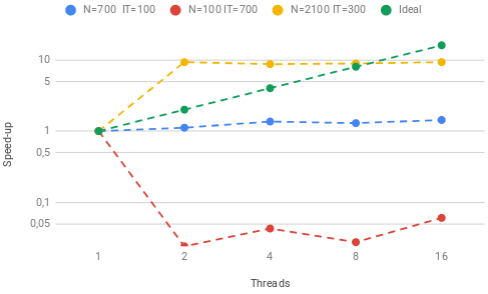
\includegraphics[width=300px]{speedup.png}
    \caption{Ganho}
\end{figure}

A observação das retas(e medições) obtidas permite retirar duas conclusões do comportamento do código em causa:
\begin{itemize}
    \item A versão sequencial do algoritmo apresenta melhor desempenho em casos em que o número de iterações é consideravelmente superior à ordem da matriz
    \item A versão paralela do algoritmo apresenta melhor desempenho para matrizes de maiores dimensões.
\end{itemize}
Os comportamentos apresentados podem ser justificados tendo por base os blocos sequenciais/paralelos presentes no algoritmo.
Em relação ao efeito do número de iterações no desempenho das duas versões, nomeadamente no melhor desempenho da versão sequencial face à paralela, é de realçar que o aumento no número de iterações corresponde a um aumento direto da percentagem do código total que é executado de maneira sequencial.
Por oposição, o melhor desempenho da versão paralela para matrizes de maiores dimensões deve-se ao paralelismo inerente a este bloco de código, que permite que o mesmo beneficie do aumento no número de \textit{threads} que o executam.

A não escalabilidade do código a partir de 2 threads apresenta várias causas.
Uma destas (no caso N=100 e IT=700) passa pela sincronização exigida ao fim de cada iteração do loop mais exterior, que é executado sequencialmente.

Já a escalabilidade super linear obtida no caso em que N=2100 e IT=300 justifica-se devido ao uso da \textit{cache} para armazenar os valores usados no cálculo do stencil, visto a localidade temporal e espacial presente no acesso aos mesmos. No entanto este comportamento super linear não se verifica para um número de threads superior a 2, algo que pode ser justificado pela partilha da cache por parte das diferentes threads que estarão a competir pela memória disponível o que leva a um aumento do número de misses nos acessos à memória bem como pela percentagem de código sequencial que limita o desempenho.

\section{Conclusões}
Os resultados obtidos permitem concluir que para matrizes de grandes dimensões(cerca de 2000 por 2000) existe um benefício em usar a versão paralela face à versão sequencial contudo, sempre limitado pela percentagem de código sequencial existente. Por outro lado, para matrizes de pequenas dimensões, independentemente do número de iterações, o mais recomendado é o uso da versão sequencial.

\end{document}